\scanpage{170}
\uline{Foncteurs \unsure{fibres|fibrés} motiviques, et gps fondamen\unsure{taux} motiviques.}

À examiner :

0)\quad VA
\figure{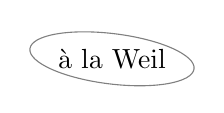
\begin{tikzpicture}[baseline=(w.base)]\node (w) at (0,0) {à la Weil};\draw[gray] (0,0) ellipse [x radius=1.05,y radius=.32,rotate=-7];\end{tikzpicture}}
\unsure{associées} aux motifs purs de poids impairs sur
\inserted{Conditions de Hodge-Riemann\ldots}

\margin{OK\quad *}
\figure{
\begin{tikzpicture}\node[draw,circle,inner sep=3pt] {1};\end{tikzpicture}}
Extension du groupe \unsure{définie|définies|défini} par des \unsure{places arithmétiques|places antiques}

\uline{Groupe fondamental motivique.}

\figure{
\begin{tikzpicture}\node[draw,circle,inner sep=3pt] {2};\end{tikzpicture}}
Relations avec le corps de classes

\margin{OK}
\figure{
\begin{tikzpicture}\node[draw,circle,inner sep=3pt] {3};\end{tikzpicture}}
Cas du spectre d'un corps fini. Pb \unsure{motivique}

\unsure{parties|positives} à \unsure{val.} dans $\mathbb{R}$ ???

\margin{*}
4)\quad Rôle du groupe fondamental motivique pour la comparaison des réseaux canoniques
\diagram{$\left[\begin{array}{ll}
\text{des \unsure{Ch.|Coh.} de Hodge} & \left|\begin{array}{l}
\text{2 réseaux \unsure{transcendant|transcendants} \unsure{pr.|prov.} des places diff.}\\
\text{réseau transcendant et \unsure{réseau|réseaux} de Hodge}
\end{array}\right.\\[1em]
\text{des Coh. $l$-adique} & \left|\text{2 réseaux transcendants}\right.
\end{array}\right]$}

5)\quad Relations \inserted{de 4} avec \unsure{mes|les} \unsure{autres} \unsure{anciens|axiomes}

6)\quad Fonctions $L$: équation fonctionnelle

\margin{OK}
7)\quad Structures \unsure{pratiques|positives|p-adiques}\ldots

\deleted{\unsure{7}}8)\quad Topologie à mettre sur $\mathbb{Z}$ \texttt{-{}-{}-{}-}

9)\quad Hyp. de Riemann \unsure{??}

\margin{Positivité à la Hodge en se ramenant à des questions de \uline{diviseurs} par \unsure{éclatements}, ou variétés de drapeaux ??}
% archive sheet number: 169
